%%Plantilla para la entrega de trabajos
\documentclass{article}
\usepackage{graphicx} %%Estos son paquetes de imagenes
\usepackage[utf8]{inputenc} %%Paquete para simbolos utf8
\usepackage[T1]{fontenc} %%Paquete para la impresion de simbolos y carácteres
\usepackage{hyperref} %%Paquete para manejar hipervinculos
\usepackage[spanish]{babel} %%paquete para el lenguaje
\usepackage{enumerate}
\usepackage{anysize} %%Margenes
\usepackage{amsmath}
\usepackage{amssymb}
\usepackage[usenames]{color}
\usepackage{float}
\author{Barajas Figueroa José de Jesús}
%%\setlength{\parindent}{1cm} %%Especificar sangrias

\begin{document}
\marginsize{3cm}{2cm}{2cm}{2cm} 
\begin{titlepage} %%Inicio de página de presentación
\begin{center}
    
\begin{figure}[ht]
\begin{center}

\includegraphics[width=1.8in]{./img/unamlogo.png}
\end{center}
\end{figure}

\begin{center}
  {\Large \textbf{
      \vspace*{.5in}   
UNIVERSIDAD NACIONAL AUTONOMA DE MEXICO\\
\vspace*{.3in}
FACULTAD DE CIENCIAS}}\\
\vspace*{.3in}
Proyecto Final\\%%nombre del trabajo
\vspace*{.3in}
Fundamentos de Bases de Datos\\
\vspace*{.3in}
Profesor: Gerardo Aviles Rosas\\
Ayudante: Maria del Pilar Hernández Bastida\\
Ayudante: Eduardo \\
Ayudamte: Eduardo \\
\vspace*{.3in}

Barajas Figueroa José de Jesús\\
Ramírez García Diana Isabel\\
\vspace*{.3in}
2019-1 \\%%Fecha
\begin{figure}[H]
\begin{center}

\includegraphics[width=2.5in]{./img/logo.png}
\end{center}
\end{figure}
\end{center}
\end{center}
\end{titlepage}
\section{Diagrama E/R}
El primer boceto de el diagrama lo hicimos prácticamente considerando las entidades y relaciones que nos proporcionaban 
de manera casi literal, esto para ir tomando consideraciones que de primer mano no son tan aproximadas como el diagrama final 
que queremos, por ahora creo que nos tenemos que concentrar en guardar lo mas posible la integridad referencial.\\ 
Decidimos no utilizar herencia en Cliente porque a pesar de tener 3 tipos diferentes de clientes, no varían en sus atributos por lo
que no es necesario utilizar la herencia.Podíamos utlilizar la herencia en las entidades Chofer y Dueño porque  en este caso
la entidad padre sería chofer porque en el caso de uso se nos especifíca que Dueño tiene los mismos atributos más su rfc, sin emabargo
decidimos no utilizarla y en su luagr crear una relación para especificar si un chofer es dueño con la finalidad de facilitar su conversión
al modelo Relacional.\\
\begin{figure}[H]
\begin{center}
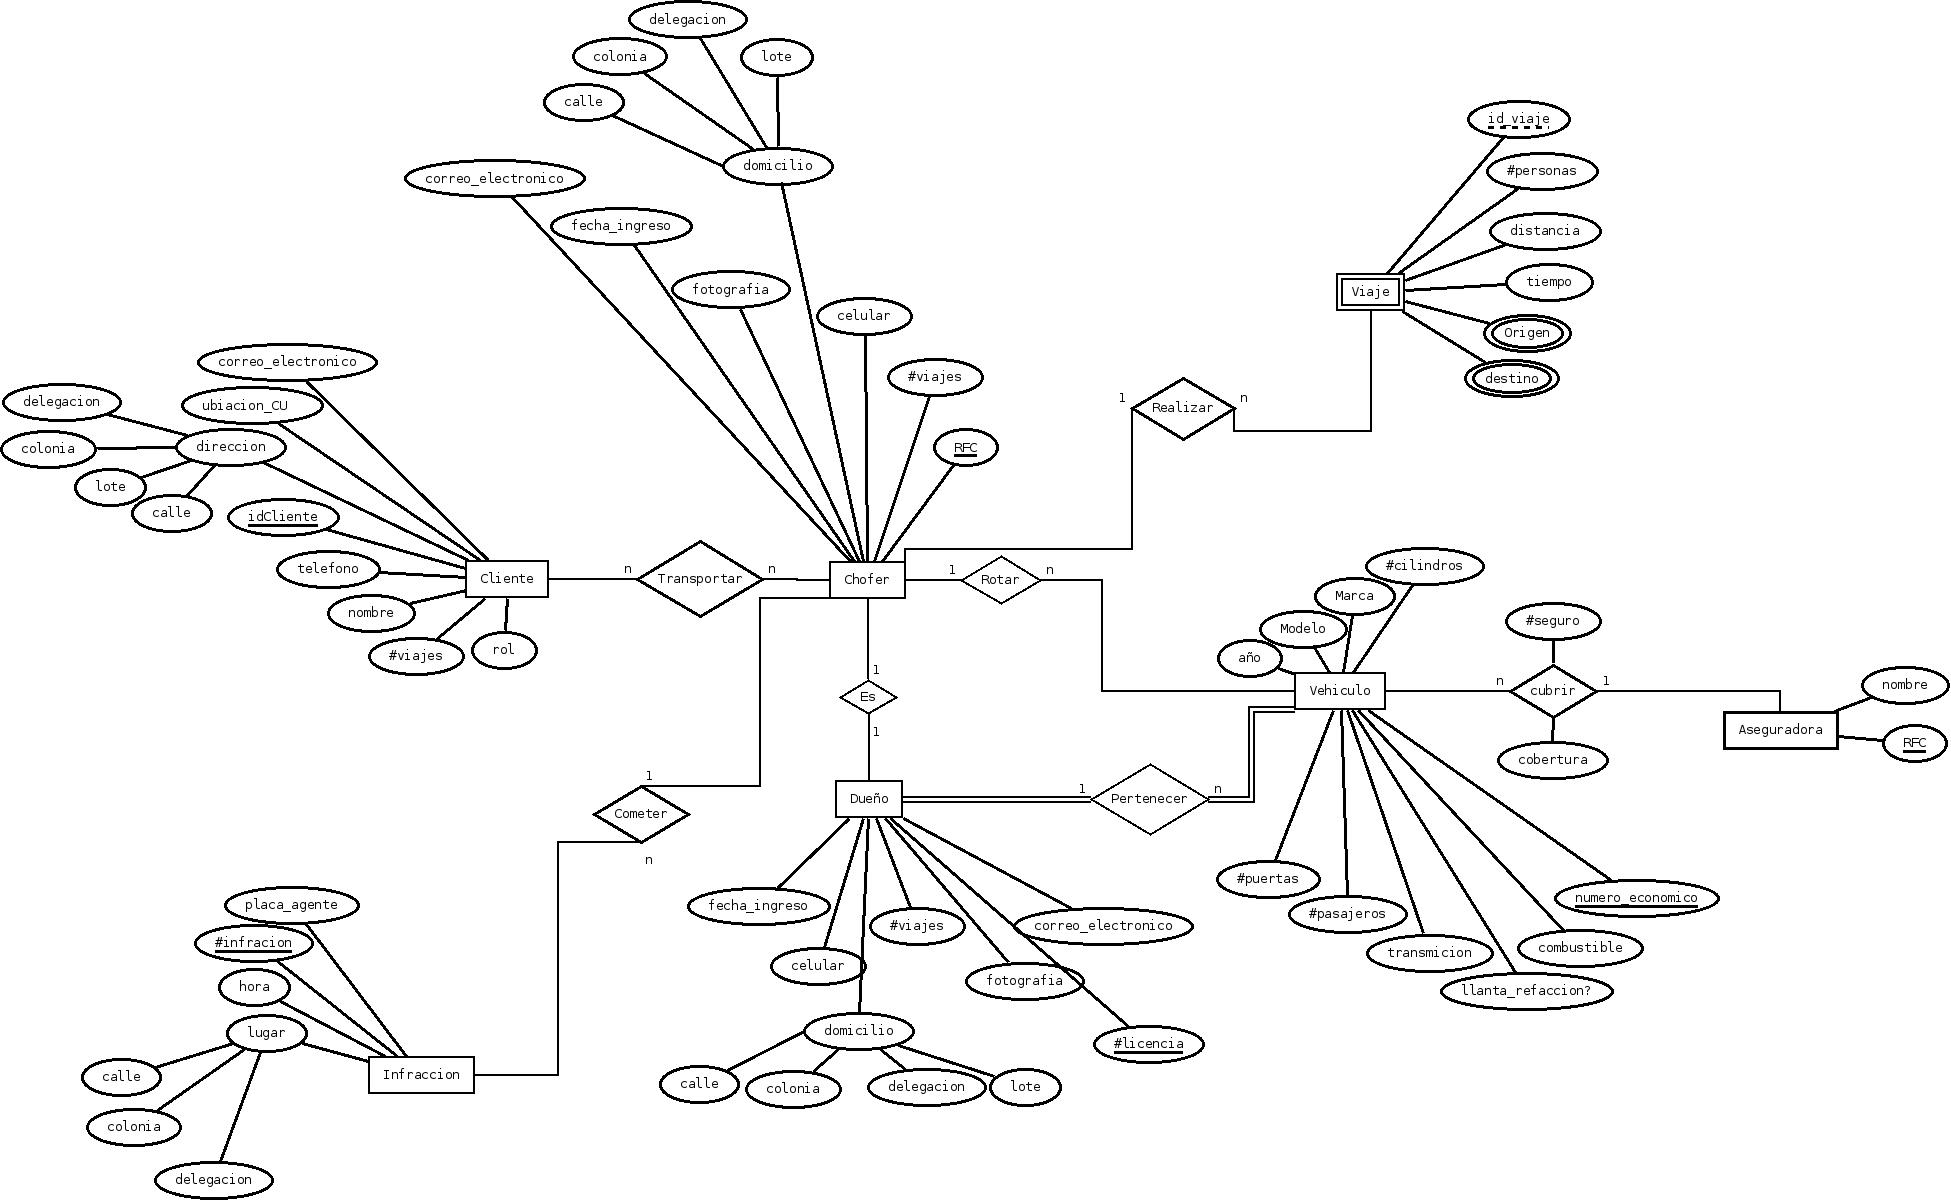
\includegraphics[width=5in]{./img/R_boceto1.jpeg}
\caption{Primer revisión 12-noviembre-2018}
\end{center}
\end{figure}
Aqui podemos observar las primeras modificaciones echas al diagrama, en primera instancia, 
convertimos la relacion transportar en una relacion ternaria, con cliente, viaje y chofer, 
ya que anteriormente teniamos viaje y clientes separados, no teniamos una forma de crear un vínculo entre el viaje y el cliente,
a su vez, dejamos intactas las relaciones, perteneces, cubrir, manejar y cometer. 
Sin embargo aun tenemos un poco de duas a cerca de como se quiera manejar el descuento de cada viaje.\\
\begin{figure}[H]
\begin{center}
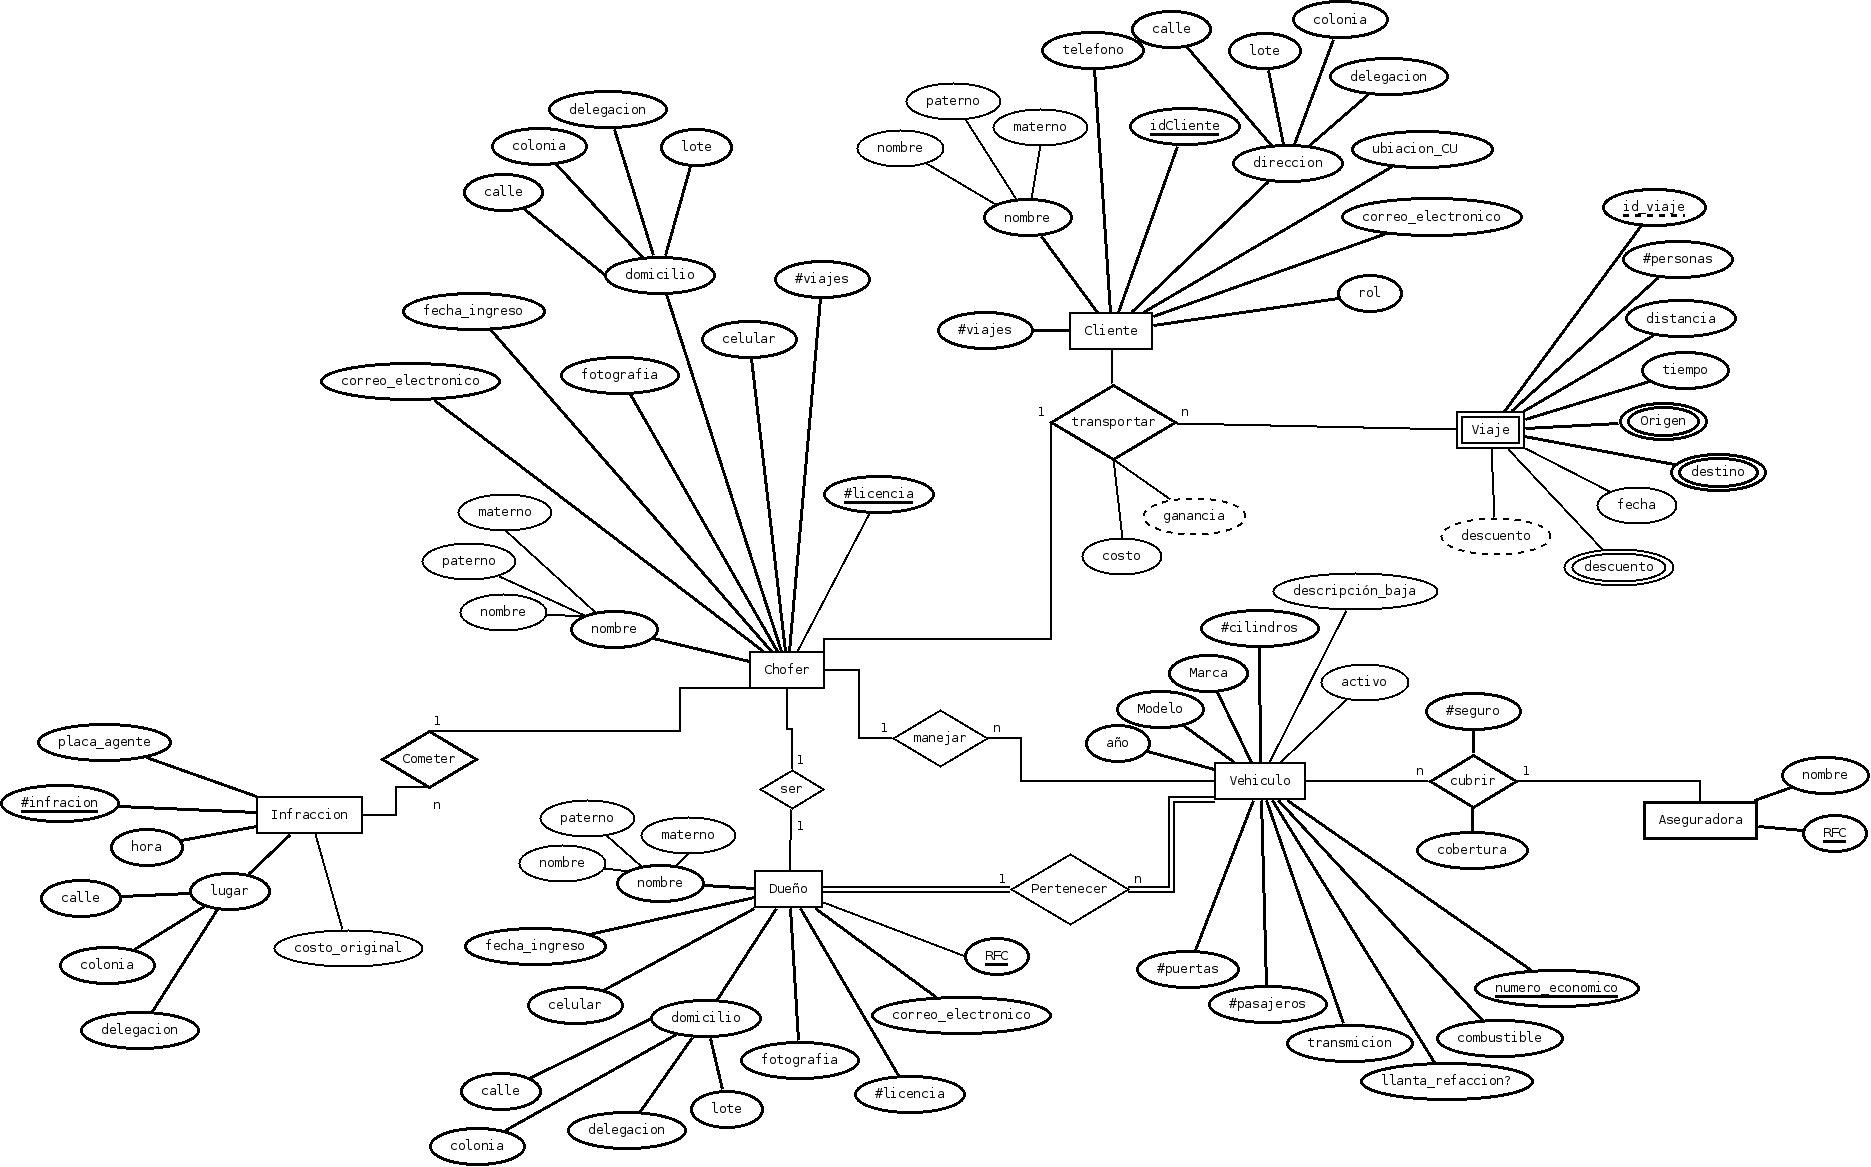
\includegraphics[width=5in]{./img/R_boceto2.jpeg}
\caption{Segunda revisión 19-Noviembre-2018}
\end{center}
\end{figure}
\begin{figure}[H]
\begin{center}
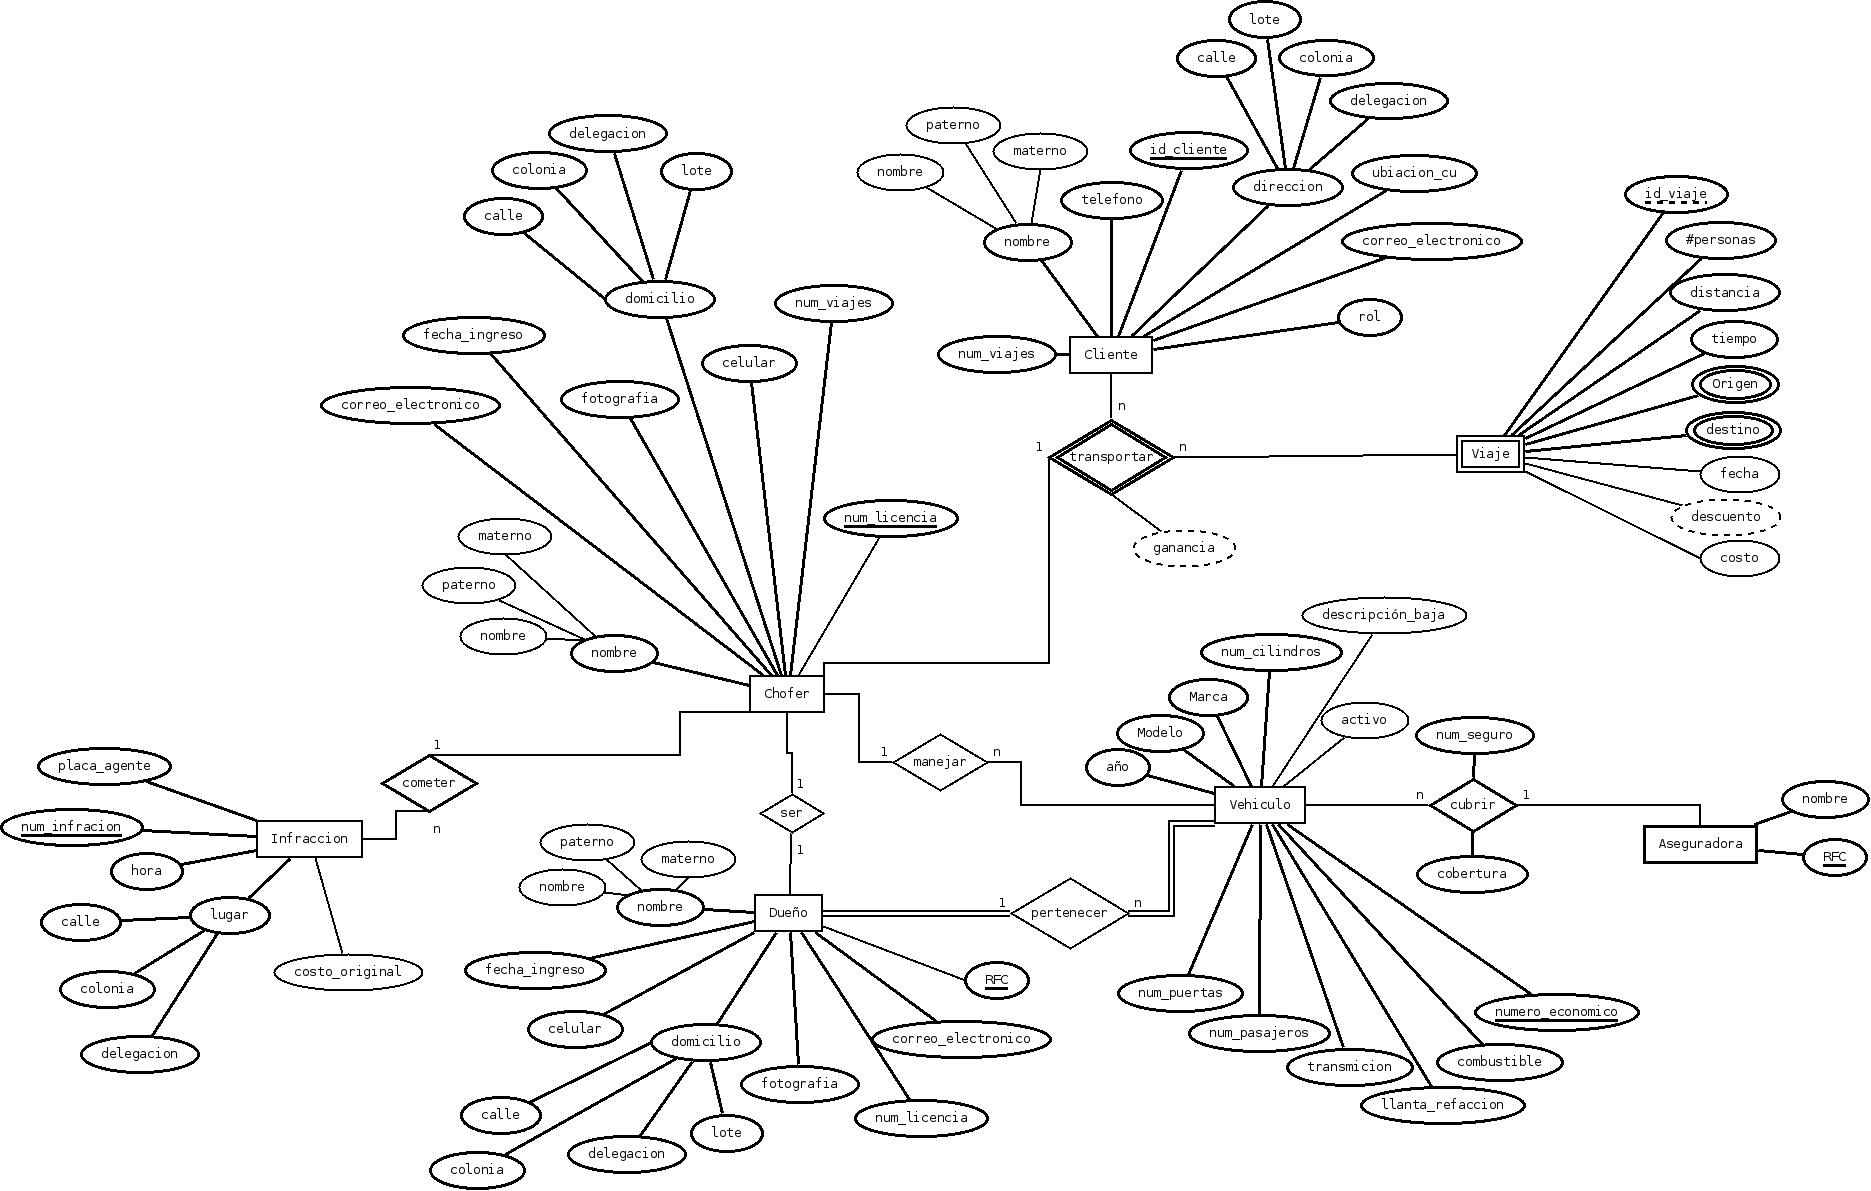
\includegraphics[width=5in]{./img/R_boceto3.jpeg}
\caption{Diagrama E/R final. 21-Noviembre-2018 }
\end{center}
\end{figure}
En esta nueva versión del diagrama, cambiamos todos los nombres de atributos que tenían símbolos especiales como \# o ?,
definimos también la relación débil,  quitamos unos atributos, por último decidimos tomar a descuento como un atributo calculado.\\
\begin{figure}[H]
\begin{center}
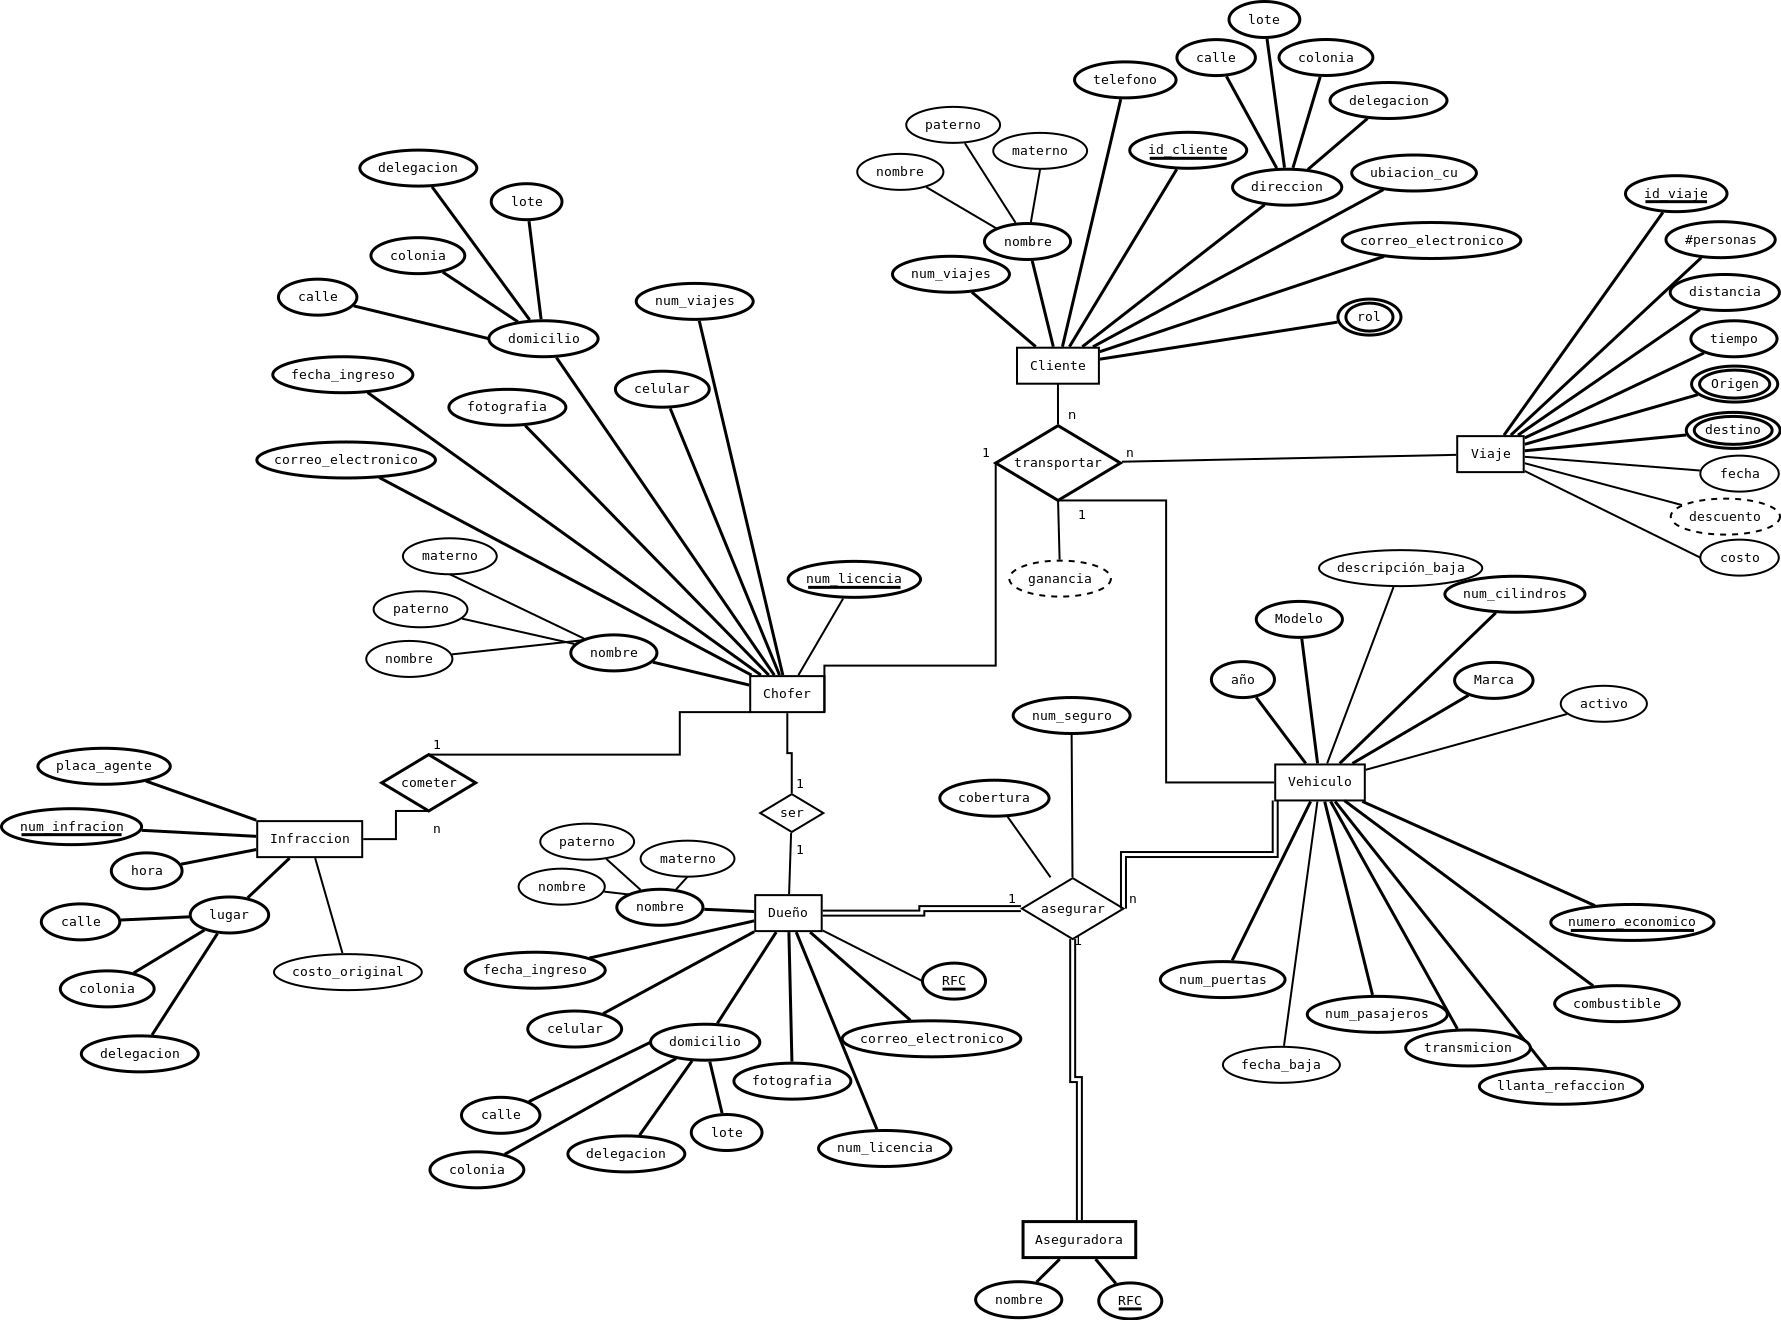
\includegraphics[width=5in]{./img/R_boceto4.png}
\caption{Diagrama E/R final. 26-Noviembre-2018 }
\end{center}
\end{figure}
En esta última versión del diagrama , cambiamos la relación transportar por una relación de grado 4 , al relacionar de igual manera 
a la entidad vehículo porque deseamos saber que coche se utilizó en el viaje,debido a que un Chofer puede manejar distintos autos y 
anteriormente no nos era posible tener esta información con las relaciones que ya teníamos.
Como consecuencia de esto quitamos la relación manejar ya que con transportar podemos conoces que vehículo y cuantos maneja un chofer.
De igual manera decidimos que Viaje fuese una entidad fuerte y de igual manera la relación transportar.Otro cambió que realizamos fue 
cambiar la cardinalidad de asegurar y la volvimos ternaria en la cual agregamos a la entidad Dueño.
\section {Diagrama Relacional}
Una vez completado el diagrama entidad relación, se comenzó con la transformación sintáctica a un diagrama Relacional, 
se aprecia el como se desaparecen los atributos calculados(datos que podemos obtener en tiempo constante sin necesidad de ocupar espacio en la base de datos).
Como es el caso de descuento, ganancia y costo, y nuestro atributos multivaluados generan nuevas tablas como lo son origen , destino y rol.\\
\begin{figure}[H]
\begin{center}
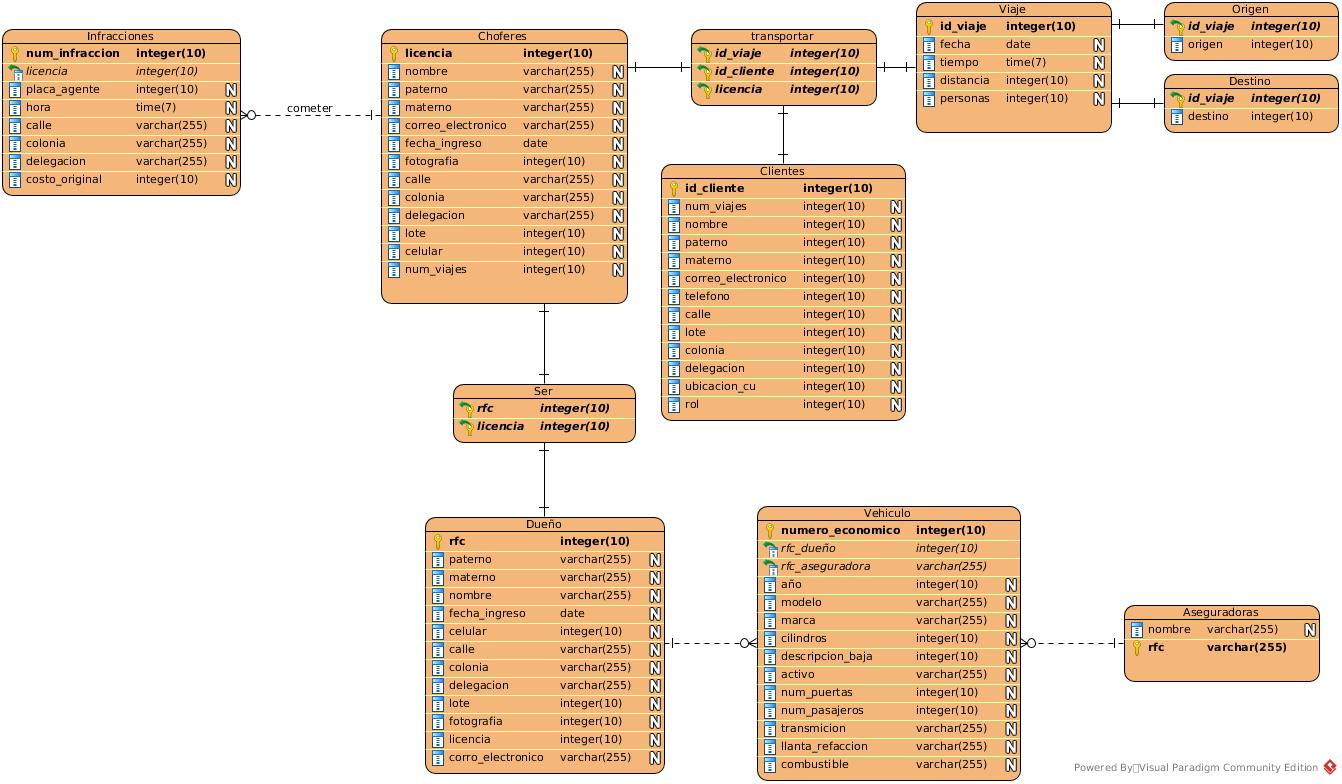
\includegraphics[width=5in]{./img/relacional.jpg}
\caption{Diagrama relacional 21-Noviembre-2018}
\end{center}
\end{figure}


\section{Normalización}
En esta sección vamos a realizar el proceso de normalización mediante la 3FN.\\
\begin{itemize}
\item 
Infracción\\ Sea Infracción (num\_infracción,licencia,costo,delegación,colonia,calle,lote).\\
Para facilitar la normalización renombraremos los atributos como sigue:
num\_infracción = A, licencia = B, costo = C, delegación = D, colonia = E , calle = F y lote = G.\\
Sea Infracción(A,B,C,D,E,F) con las dependencias funcionales 
Infracción = \{A $\rightarrow$ CB, D $\rightarrow$ EF \} \\
\\
Buscamos atributos superfluos iquierdos:\\
No tenemos dependencias para buscar elementos superfluos izquierdos.\\
\\
Buscamos atributos superfluos derechos:\\
Sea A $\rightarrow$ CB \\
¿C es superfluo? $\Rightarrow$ A $\rightarrow$ B \\
\{A\}+= \{A,B\} No aparece C, entonces no es superfluo.\\
¿B es superfluo? $\Rightarrow$ A $\rightarrow$ C \\
\{A\}+= \{A,C\} No aparece B, entonces no es superfluo.\\
\\
Sea D $\rightarrow$ EFG\\
¿E es superfluo? $\Rightarrow$ D $\rightarrow$ F \\
\{D\}+= \{D,F,G\} No aparece E, entonces no es superfluo.\\
¿F es superfluo? $\Rightarrow$ D $\rightarrow$ E \\
\{D\}+= \{D,E,G\} No aparece F, entonces no es superfluo.\\
¿F es superfluo? $\Rightarrow$ D $\rightarrow$ E \\
\{D\}+= \{D,E,F\} No aparece G, entonces no es superfluo.\\
\\
Sea Fmin = \{A $\rightarrow$ CB, D $\rightarrow$ EF\}\\
Tendremos las siguientes relaciones resultantes:
\begin{itemize}
\item Infracción(num\_infraccion,licencia,costo)
\item Dirección(delegación,colonia,calle,lote)
\end{itemize}

\item Chofer\\
Sea Chofer(licencia,nombre,paterno,materno,correo\_electronico,fecha\_ingreso,fotografia,delegación,colonia,calle,lote,celular,num\_viajes).\\
Para facilitar la normalización renombraremos los atributos como sigue:
licencia = A,nombre = B,paterno = C,materno = D,correo\_electronico = E,fecha\_ingreso = F,fotografia = G,delegación = H,colonia = I,calle = J,lote = K,celular = L,num\_viajes = M\\
Sea Chofer(A,B,C,D,E,F,G,H,I,J,K,L,M) con las dependencias funcionales 
Infracción = \{A $\rightarrow$ BCDEFGLM, H $\rightarrow$ IJK  \} \\
\\
Buscamos atributos superfluos iquierdos:\\
No tenemos dependencias para buscar elementos superfluos izquierdos.\\
Buscamos atributos superfluos derechos:\\
\\
Sea A $\rightarrow$ BCDEFGLM\\
¿C es superfluo? $\Rightarrow$ A $\rightarrow$ BDEFGLM \\
\{A\}+= \{A,B,D,E,F,G,L,M\} No aparece C, entonces no es superfluo.\\
¿B es superfluo? $\Rightarrow$ A $\rightarrow$ CDEFGLM \\
\{A\}+= \{A,C,D,E,F,G,L,M\} No aparece B, entonces no es superfluo.\\
¿D es superfluo? $\Rightarrow$ A $\rightarrow$ BCEFGLM \\
\{A\}+= \{A,B,C,E,F,G,L,M\}  No aparece D, entonces no es superfluo.\\
¿E es superfluo? $\Rightarrow$ A $\rightarrow$ BCDFGLM \\
\{A\}+= \{A,B,C,D,F,G,L,M\}  No aparece E, entonces no es superfluo.\\
¿F es superfluo? $\Rightarrow$ A $\rightarrow$ BCDEGLM \\
\{A\}+= \{A,B,C,D,E,G,L,M\}  No aparece F, entonces no es superfluo.\\
¿G es superfluo? $\Rightarrow$ A $\rightarrow$ BCDEFLM \\
\{A\}+= \{A,B,C,D,E,F,L,M\}  No aparece G, entonces no es superfluo.\\
¿L es superfluo? $\Rightarrow$ A $\rightarrow$ BCDEFGM \\
\{A\}+= \{A,B,C,D,E,F,G,M\}  No aparece L, entonces no es superfluo.\\
¿M es superfluo? $\Rightarrow$ A $\rightarrow$ BCDEFGL \\
\{A\}+= \{A,B,C,D,E,F,G,L\}  No aparece M, entonces no es superfluo.\\
\\
Sea H $\rightarrow$ IJK 
¿I es superfluo? $\Rightarrow$ H $\rightarrow$ JK \\
\{H\}+= \{H,J,K\} No aparece I, entonces no es superfluo.\\
¿J es superfluo? $\Rightarrow$ H $\rightarrow$ IK \\
\{H\}+= \{H,J,K\} No aparece J, entonces no es superfluo.\\
¿K es superfluo? $\Rightarrow$ H $\rightarrow$ IJ \\
\{H\}+= \{H,I,J\} No aparece K, entonces no es superfluo.\\
\\
Sea Fmin = \{A $\rightarrow$ BCDEFGLM, H $\rightarrow$ IJK  \}\\
Tendremos las siguientes relaciones resultantes:
\begin{itemize}
\item Chofer(licencia,nombre,paterno,materno,correo\_electronico,fecha\_ingreso,fotografia,celular,num\_viajes)
\item Dirección(delegación,colonia,calle,lote)
\end{itemize}

\item Ser\\
Sea Ser(rfc,licencia)
Para facilitar la normalización renombraremos los atributos como sigue:
rfc= A y licencia = B
Sea Ser(A,B) con las dependencias funcionales 
Ser = \{AB $\rightarrow$ AB\} \\
\\
Tenemos una única dependencia funcional trivial, ya esta normalizada.
Sea Fmin = \{AB $\rightarrow$ AB\} \\
Tendremos las siguientes relaciones resultantes:
\begin{itemize}
\item Ser(rfc,licencia)
\end{itemize}


\item Dueño\\
Sea Dueño(licencia,nombre,paterno,materno,correo\_electronico,fecha\_ingreso,fotografia,delegación,colonia,calle,lote,celular,num\_viajes,rfc).\\
Para facilitar la normalización renombraremos los atributos como sigue:
licencia = N,nombre = B,paterno = C,materno = D,correo\_electronico = E,fecha\_ingreso = F,fotografia = G,delegación = H,colonia = I,calle = J,lote = K,celular = L,num\_viajes = M, rfc = A\\
Sea Dueño(A,B,C,D,E,F,G,H,I,J,K,L,M,N) con las dependencias funcionales 
Dueño = \{A $\rightarrow$ BCDEFGLMN, H $\rightarrow$ IJK  \} \\
\\
Buscamos atributos superfluos iquierdos:\\
No tenemos dependencias para buscar elementos superfluos izquierdos.\\
Buscamos atributos superfluos derechos:\\
\\
Sea A $\rightarrow$ BCDEFGLMN\\
¿C es superfluo? $\Rightarrow$ A $\rightarrow$ BDEFGLMN \\
\{A\}+= \{A,B,D,E,F,G,L,M,N\} No aparece C, entonces no es superfluo.\\
¿B es superfluo? $\Rightarrow$ A $\rightarrow$ CDEFGLMN \\
\{A\}+= \{A,C,D,E,F,G,L,M,N\} No aparece B, entonces no es superfluo.\\
¿D es superfluo? $\Rightarrow$ A $\rightarrow$ BCEFGLMN \\
\{A\}+= \{A,B,C,E,F,G,L,M,N\}  No aparece D, entonces no es superfluo.\\
¿E es superfluo? $\Rightarrow$ A $\rightarrow$ BCDFGLMN \\
\{A\}+= \{A,B,C,D,F,G,L,M,N\}  No aparece E, entonces no es superfluo.\\
¿F es superfluo? $\Rightarrow$ A $\rightarrow$ BCDEGLMN \\
\{A\}+= \{A,B,C,D,E,G,L,M,N\}  No aparece F, entonces no es superfluo.\\
¿G es superfluo? $\Rightarrow$ A $\rightarrow$ BCDEFLMN \\
\{A\}+= \{A,B,C,D,E,F,L,M,N\}  No aparece G, entonces no es superfluo.\\
¿L es superfluo? $\Rightarrow$ A $\rightarrow$ BCDEFGMN \\
\{A\}+= \{A,B,C,D,E,F,G,M,N\}  No aparece L, entonces no es superfluo.\\
¿M es superfluo? $\Rightarrow$ A $\rightarrow$ BCDEFGLN \\
\{A\}+= \{A,B,C,D,E,F,G,L,N\}  No aparece M, entonces no es superfluo.\\
¿N es superfluo? $\Rightarrow$ A $\rightarrow$ BCDEFGLM \\
\{A\}+= \{A,B,C,D,E,F,G,L,M\}  No aparece M, entonces no es superfluo.\\
\\
Sea H $\rightarrow$ IJK 
¿I es superfluo? $\Rightarrow$ H $\rightarrow$ JK \\
\{H\}+= \{H,J,K\} No aparece I, entonces no es superfluo.\\
¿J es superfluo? $\Rightarrow$ H $\rightarrow$ IK \\
\{H\}+= \{H,J,K\} No aparece J, entonces no es superfluo.\\
¿K es superfluo? $\Rightarrow$ H $\rightarrow$ IJ \\
\{H\}+= \{H,I,J\} No aparece K, entonces no es superfluo.\\
\\
Sea Fmin = \{A $\rightarrow$ BCDEFGLMN, H $\rightarrow$ IJK  \}\\
Tendremos las siguientes relaciones resultantes:
\begin{itemize}
\item Dueño(licencia,nombre,paterno,materno,correo\_electronico,fecha\_ingreso,fotografia,celular,num\_viajes,rfc)
\item Dirección(delegación,colonia,calle,lote)
\end{itemize}


\item Vehículo\\
Sea Vehículo(número\_económico,año,modelo,marca,cilindros,descripción\_baja,activo
,num\_puertas, num\_pasajeros, transmición,llanta\_refacción,combustible,fecha\_baja)\\
Para facilitar la normalización renombraremos los atributos como sigue:
número\_económico = A,año,modelo = B,marca,cilindros = C,descripción\_baja = D,activo = E
,num\_puertas = F, num\_pasajeros = G, transmición = H,llanta\_refacción = I,combustible = J,fecha\_baja = K
Sea Vehículo(A,B,C,D,E,F,G,H,I,J,K) con las dependencias funcionales
Vehículo(A $\rightarrow$ ) \\
\\



\item Aseguradora\\
Sea Aseguradora(rfc,nombre)\\
Para facilitar la normalización renombraremos los atributos como sigue:
rfc = A y nombre = B.\\
Sea Aseguradora(A,B) con las dependencias funcionales 
Dueño = \{A $\rightarrow$ B\} \\
\\
Tenemos una única dependencia funcional trivial, ya esta normalizada.
Tendremos las siguientes relaciones resultantes:
\begin{itemize}
\item Aseguradora(rfc,nombre)\\
\end{itemize}


\item Asegurar\\
Sea Asegurar(dueño\_rfc,aseguradora\_rfc, vehiculo\_numero\_económico, num\_seguro,cobertura)\\
Para facilitar la normalización renombraremos los atributos como sigue:
dueño\_rfc = A,aseguradora\_rfc = B, vehiculo\_numero\_económico = C, num\_seguro = D,cobertura = E\\
Sea Asegurar(A,B,C,D,E) con las dependencias funcionales 
Asegurar = \{ABC $\rightarrow$ DE\} \\
\\


\item Viaje\\
Sea Viaje(id\_viaje,fecha,tiempo,distancia,personas)\\
Para facilitar la normalización renombraremos los atributos como sigue:
id\_viaje = A,fecha = B,tiempo = C,distancia = D,personas = E.\\
Sea Viaje(A,B,C,D,E) con las dependencias funcionales
Asegurar = \{A $\rightarrow$ BCDE\} \\
\\



\item Destino\\
Sea Destino(id\_viaje,destino)\\
Para facilitar la normalización renombraremos los atributos como sigue:
id\_viaje = A y destino = B.\\
Sea Viaje(A,B) con las dependencias funcionales
Viaje = \{A $\twoheadrightarrow$ B\} \\
\\
Tenemos una única dependencia funcional trivial, ya esta normalizada.
Tendremos las siguientes relaciones resultantes:
\begin{itemize}
\item Destino(id\_viaje,destino)\\
\end{itemize}

\item Origen\\
Sea Origen(id\_viaje,origen)\\
Para facilitar la normalización renombraremos los atributos como sigue:
id\_viaje = A y origen = B.\\
Sea Viaje(A,B) con las dependencias funcionales
Viaje = \{A $\twoheadrightarrow$ B\} \\
\\
Tenemos una única dependencia funcional trivial, ya esta normalizada.
Tendremos las siguientes relaciones resultantes:
\begin{itemize}
\item Sea Origen(id\_viaje,origen)\\
\end{itemize}

\item Cliente\\
Sea Cliente(id_cliente,nombre,paterno,materno,correo\_electronico,delegación,colonia,calle,lote,telefono,num\_viajes,ubicación\_cu)\\
Para facilitar la normalización renombraremos los atributos como sigue:
id_cliente = A,nombre = B,paterno = C,materno = D,correo\_electronico = E,delegación = F,colonia = G,calle = H,lote = I,telefono = J,num\_viajes = K,ubicación\_cu = L.\\
Sea Cliente(A,B,C,D,E,F,G,H,I,J,K,L) con las dependencias funcionales
Cliente = \{A $\rightarrow$ BCDEKL, F $\rightarrow$ GHI  \} \\
\\

\item Rol\\
Sea Rol(cliente\_id, rol)\\
Para facilitar la normalización renombraremos los atributos como sigue:
cliente\_id = A y rol = B.\\
Sea Viaje(A,B) con las dependencias funcionales
Viaje = \{A $\twoheadrightarrow$ B\} \\
\\
Tenemos una única dependencia funcional trivial, ya esta normalizada.
Tendremos las siguientes relaciones resultantes:
\begin{itemize}
\item Sea Rol(cliente\_id, rol)\\
\end{itemize}

\item Transportar\\
Sea Transportar(id\_viaje,id\_cliente,licencia,vehiculo\_numero\_economico)\\
Para facilitar la normalización renombraremos los atributos como sigue:
id\_viaje = A,id\_cliente = B,licencia = C,vehiculo\_numero\_economico = D.\\
Sea Transportar(A,B,C,D) con las dependencias funcionales
Transportar = \{ABCD $\rightarrow$ ABCD \} \\
\\


\end{itemize}
Después de normalizar tendremos las siguientes relaciones:
\begin{itemize}
\item Infracción\\
\item Chofer\\
\item Ser\\
\item Dueño\\
\item Vehículo\\
\item Asegurar\\
\item Aseguradora\\
\item Viaje\\
\item Destino\\
\item Origen\\
\item Cliente\\
\item Rol\\
\item Transportar\\
\item Dirección\\

\end{itemize}




\section{Referencias}

\end{document}
